\section{Documentos y Ejecutables}
\subsection{Game Design Document}

\subsection{Repositorios}
\begin{itemize}
  \item EcoRescue: \url{https://github.com/dexaxi/RecursosSolarcore}
  \item DUJAL: \url{https://github.com/dexaxi/TFG\textunderscore Unity\textunderscore Package}
  \item AkyuiUnity: \url{https://github.com/kyubuns/AkyuiUnity/tree/main} 
  \item AnKuchen: \url{https://github.com/kyubuns/AnKuchen}
  \item Auto9Slicer: \url{https://github.com/kyubuns/Auto9Slicer}
  \item UniTask: \url{https://github.com/Cysharp/UniTask}
\end{itemize}

\subsection{Redes de EcoRescue}
Descarga el juego: \url{https://dexaxi.itch.io/eco-rescue}

Disponible en Windows, Linux, Mac, Android y WebGL

\section{Tablas y figuras}

\subsection{Resultados del Cuestionario}
% Insertar una figura
\begin{figure}[H]
  \centering
  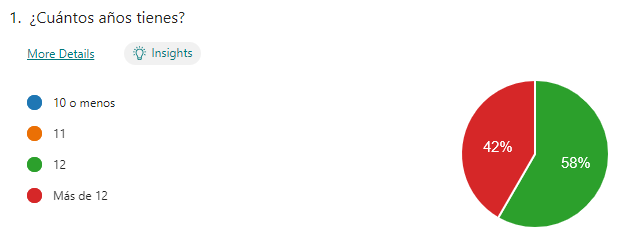
\includegraphics[width=450px,clip=true]{questionario_1.png}
  \caption{¿Cuántos años tienes?}
  \label{fig:questionario_1}
\end{figure}
\raggedbottom

\begin{figure}[H]
  \centering
  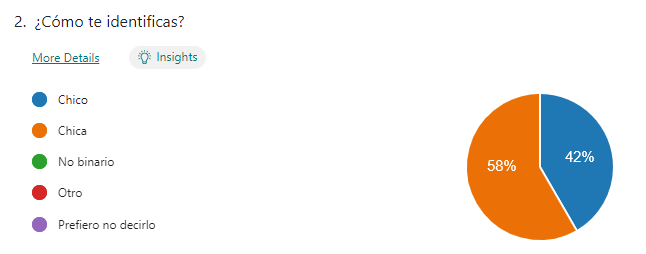
\includegraphics[width=450px,clip=true]{questionario_2.png}
  \caption{¿Cómo te identificas?}
  \label{fig:questionario_2}
\end{figure}
\raggedbottom

\begin{figure}[H]
  \centering
  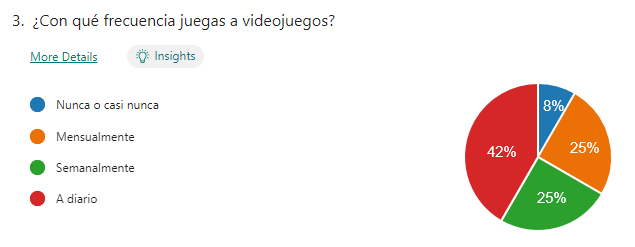
\includegraphics[width=450px,clip=true]{questionario_3.png}
  \caption{¿Con qué frecuencia juegas a videojuegos?}
  \label{fig:questionario_3}
\end{figure}
\raggedbottom

\begin{figure}[H]
  \centering
  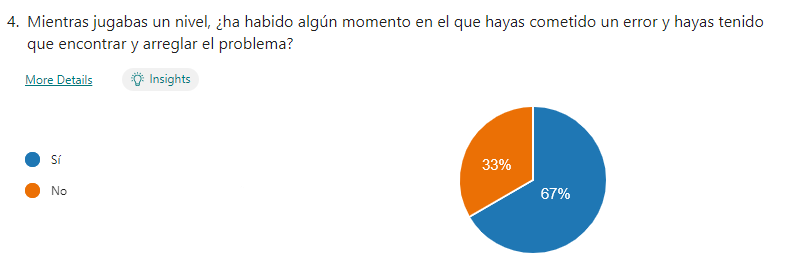
\includegraphics[width=450px,clip=true]{questionario_4.png}
  \caption{Mientras jugabas a un nivel, ¿ha habido algún momento en el que hayas cometido un error y hayas tenido que encontrar y arreglar el problema?}
  \label{fig:questionario_4}
\end{figure}
\raggedbottom

\begin{figure}[H]
  \centering
  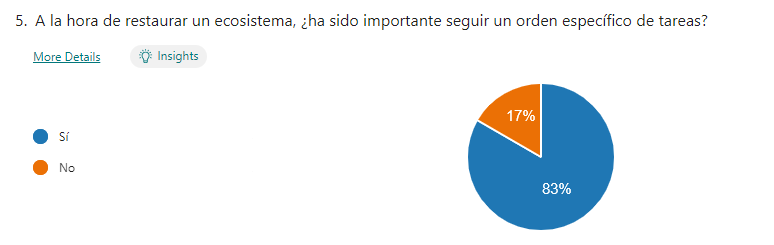
\includegraphics[width=450px,clip=true]{questionario_5.png}
  \caption{A la hora de restaurar un ecosistema, ¿Ha sido importante seguir un orden específico de tareas?}
  \label{fig:questionario_5}
\end{figure}
\raggedbottom

\begin{figure}[H]
  \centering
  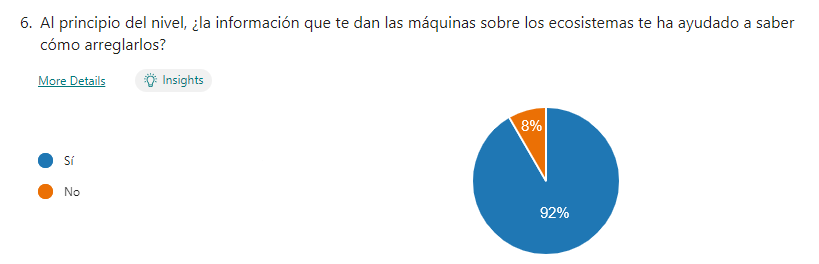
\includegraphics[width=450px,clip=true]{questionario_6.png}
  \caption{Al principio del nivel, ¿la información que te dan las máquinas sobre los ecosistemas te ha ayudado a saber cómo arreglarlos?}
  \label{fig:questionario_6}
\end{figure}
\raggedbottom

\begin{figure}[H]
  \centering
  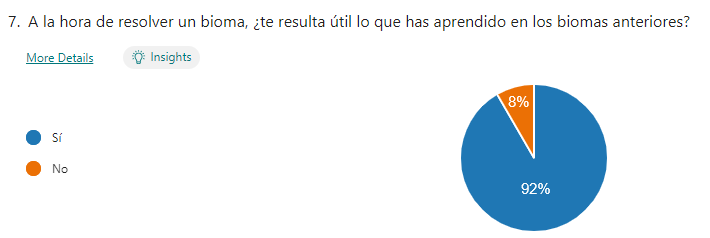
\includegraphics[width=450px,clip=true]{questionario_7.png}
  \caption{A la hora de resolver un problema, ¿te resulta útil lo que has aprendido en los biomas anteriores?}
  \label{fig:questionario_7}
\end{figure}
\raggedbottom

\begin{figure}[H]
  \centering
  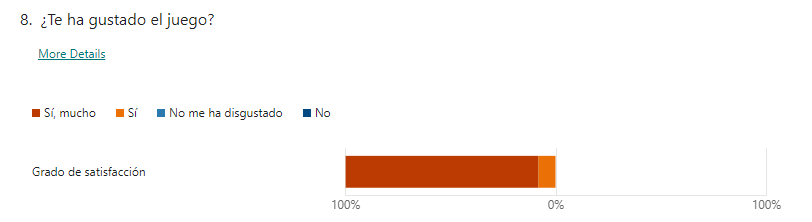
\includegraphics[width=450px,clip=true]{questionario_8.png}
  \caption{¿Te ha gustado el juego?}
  \label{fig:questionario_8}
\end{figure}
\raggedbottom

\begin{figure}[H]
  \centering
  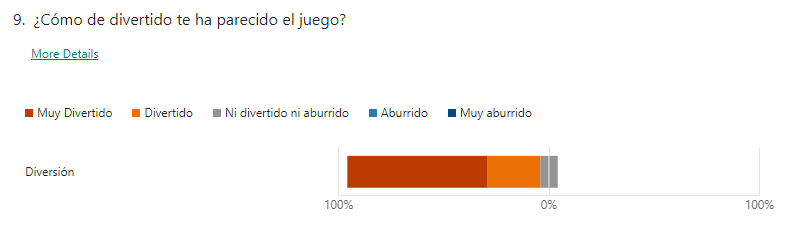
\includegraphics[width=450px,clip=true]{questionario_9.png}
  \caption{¿Cómo de divertido te ha parecido el juego?}
  \label{fig:questionario_9}
\end{figure}
\raggedbottom

\begin{figure}[H]
  \centering
  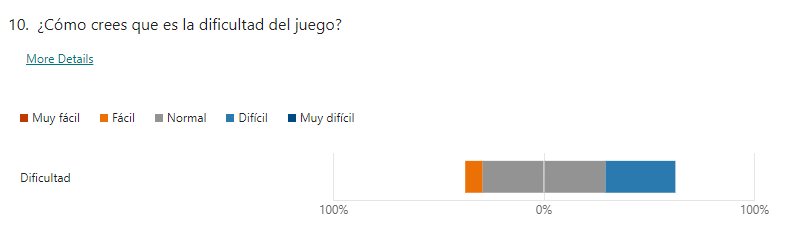
\includegraphics[width=450px,clip=true]{questionario_10.png}
  \caption{¿Cómo crees que es la dificultad del juego?}
  \label{fig:questionario_10}
\end{figure}
\raggedbottom

\begin{figure}[H]
  \centering
  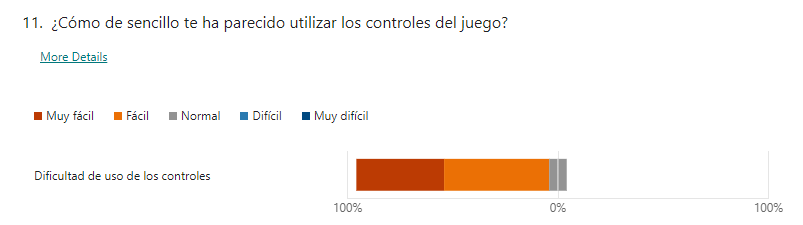
\includegraphics[width=450px,clip=true]{questionario_11.png}
  \caption{¿Cómo de sencillo te ha parecido utilizar los controles del juego?}
  \label{fig:questionario_11}
\end{figure}
\raggedbottom

\begin{figure}[H]
  \centering
  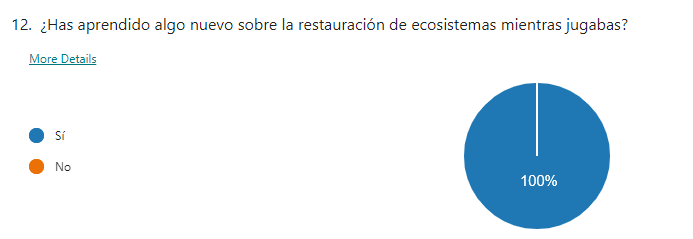
\includegraphics[width=450px,clip=true]{questionario_12.png}
  \caption{¿Has aprendido algo nuevo sobre la restauración de ecosistemas mientras jugabas?}
  \label{fig:questionario_12}
\end{figure}
\raggedbottom

\begin{table}[H]
  \begin{center}
  \setlength{\tabcolsep}{5pt}
  \renewcommand{\arraystretch}{1.2}
  \begin{tabular}{ | m{\textwidth} | } 
    \hline
    'La información que dan es muy útil' \\ 
    'He podido aprender mientras jugaba' \\ 
    'Me han gustado mucho los diseños, también me ha gustado cuando ponías las máquinas para ayudar al ecosistema' \\ 
    'La originalidad y poder aprender más sobre los ecosistemas' \\ 
    'Es fácil de usar y te explica muy bien las cosas' \\ 
    'Me ha gustado mucho la decoración y la base del juego, creo que es mucho más divertido comparado con los otros utensilios de clase' \\ 
    'Me gusta como iba subiendo la barra de progreso' \\ 
    'Las diferentes funciones de las máquinas' \\ 
    \hline
  \end{tabular}
  \centering
  \caption{¿Qué es lo que más te ha gustado del juego?}
  \label{fig:tablaResultadosPC}
  \end{center}
\end{table}  
 
\subsection{Datos Obtenidos por Telemetría}
\begin{table}[H]
  \begin{center}
  \setlength{\tabcolsep}{5pt}
  \renewcommand{\arraystretch}{1.2}
  \hspace*{-40px}
  \begin{tabular}{ @{} | m{2em} | m{4em} | m{3em} | m{2em} | m{4em} | m{4em} | m{4em} | m{3em} | m{3em} | m{4em} |  } 
  \hline
  ID & Name & Gender & Age & Progress & Machines Placed  & Machines Sold & Success Phase & Failure Phase & Duration \\
  \hline
  121  & 'Sandia' & 'Chica' &12 &0 &0 &0 &0 &0 &0  \\
  \hline
  121  & 'Sandia' & 'Chica' &12 &11 &2 &1 &1 &0 &2  \\
  \hline
  121  & 'Sandia' & 'Chica' &12 &22 &6 &4 &2 &3 &4  \\
  \hline
  121  & 'Sandia' & 'Chica' &12 &55 &9 &4 &5 &5 &6  \\
  \hline
  121  & 'Sandia' & 'Chica' &12 &100 &14 &5 &9 &9 &8  \\
  \hline
  122  & 'Ana' & 'Chica' &12 &0 &0 &0 &0 &0 &0  \\
  \hline
  122  & 'Ana' & 'Chica' &12 &22 &5 &3 &2 &2 &2  \\
  \hline
  122  & 'Ana' & 'Chica' &12 &44 &7 &3 &4 &4 &4  \\
  \hline
  122  & 'Ana' & 'Chica' &12 &100 &14 &5 &9 &9 &6  \\
  \hline
  123  & 'Ireee' & 'Chica' &13 &0 &0 &0 &0 &0 &0  \\
  \hline
  123  & 'Ireee' & 'Chica' &13 &33 &5 &2 &3 &2 &2  \\
  \hline
  123  & 'Ireee' & 'Chica' &13 &55 &8 &3 &5 &3 &4  \\
  \hline
  123  & 'Ireee' & 'Chica' &13 &100 &12 &3 &9 &5 &6  \\
  \hline
  124  & 'Bea' & 'Chica' &12 &0 &0 &0 &0 &0 &0  \\
  \hline
  124  & 'Bea' & 'Chica' &12 &33 &7 &4 &3 &2 &2  \\
  \hline
  124  & 'Bea' & 'Chica' &12 &44 &9 &5 &4 &3 &4  \\
  \hline
  124  & 'Bea' & 'Chica' &12 &100 &14 &5 &9 &5 &6  \\
  \hline
  125  & 'Leo' & 'Chico' &12 &0 &0 &0 &0 &0 &0  \\
  \hline
  125  & 'Leo' & 'Chico' &12 &22 &3 &1 &2 &0 &2  \\
  \hline
  125  & 'Leo' & 'Chico' &12 &33 &5 &2 &3 &3 &4  \\
  \hline
  125  & 'Leo' & 'Chico' &12 &55 &7 &2 &5 &4 &6  \\
  \hline
  126  & 'SALVA' & 'Chico' &13 &0 &0 &0 &0 &0 &0  \\
  \hline
  126  & 'SALVA' & 'Chico' &13 &33 &6 &3 &3 &2 &2  \\
  \hline
  126  & 'SALVA' & 'Chico' &13 &55 &8 &3 &5 &3 &4  \\
  \hline
  126  & 'SALVA' & 'Chico' &13 &100 &12 &3 &9 &5 &6  \\
  \hline
  127  & 'Calvo Pro' & 'Chico' &12 &0 &0 &0 &0 &0 &0 \\
  \hline
  127  & 'Calvo Pro' & 'Chico' &12 &22 &7 &5 &2 &1 &2 \\
  \hline 
  127  & 'Calvo Pro' & 'Chico' &12 &33 &8 &5 &3 &2 &4 \\
  \hline 
\end{tabular}
\centering
\end{center}
\end{table} 

\begin{table}[H]
  \begin{center}
  \setlength{\tabcolsep}{5pt}
  \renewcommand{\arraystretch}{1.2}
  \hspace*{-60px}
  \begin{tabular}{ @{} | m{2em} | m{4em} | m{3em} | m{2em} | m{4em} | m{4em} | m{4em} | m{3em} | m{3em} | m{4em} |  } 
  \hline
  128  & 'Virgy' & 'Chica' &12 &0 &0 &0 &0 &0 &0  \\
  \hline
  128  & 'Virgy' & 'Chica' &12 &33 &7 &4 &3 &2 &2  \\
  \hline
  128  & 'Virgy' & 'Chica' &12 &55 &9 &4 &5 &4 &4  \\
  \hline
  128  & 'Virgy' & 'Chica' &12 &100 &13 &4 &9 &5 &6  \\
  \hline
  129  & 'Sara' & 'Chica' &12 &0 &0 &0 &0 &0 &0  \\
  \hline
  129  & 'Sara' & 'Chica' &12 &33 &4 &1 &3 &2 &2  \\
  \hline
  129  & 'Sara' & 'Chica' &12 &44 &5 &1 &4 &3 &4  \\
  \hline
  129  & 'Sara' & 'Chica' &12 &100 &10 &1 &9 &7 &6  \\
  \hline
  130  & 'Paula' & 'Chica' &12 &0 &0 &0 &0 &0 &0  \\
  \hline
  130  & 'Paula' & 'Chica' &12 &11 &1 &0 &1 &1 &2  \\
  \hline
  130  & 'Paula' & 'Chica' &12 &33 &3 &0 &3 &2 &4  \\
  \hline
  130  & 'Paula' & 'Chica' &12 &77 &7 &0 &7 &6 &6  \\
  \hline
  131  & 'Pako' & 'Chico' &13 &0 &0 &0 &0 &0 &0  \\
  \hline
  132  & 'Pako' & 'Chico' &13 &22 &3 &1 &2 &1 &2  \\
  \hline
  133  & 'Pako' & 'Chico' &13 &55 &7 &2 &5 &2 &4  \\
  \hline
  134  & 'Pako' & 'Chico' &13 &66 &10 &4 &6 &5 &6  \\
  \hline
  135  & 'Pako' & 'Chico' &13 &66 &10 &4 &6 &6 &8  \\
  \hline
  136  & 'Pako' & 'Chico' &13 &66 &10 &4 &6 &7 &10  \\
  \hline
  137  & 'Pako' & 'Chico' &13 &66 &10 &4 &6 &8 &12  \\
  \hline
  138  & 'Pako' & 'Chico' &13 &66 &10 &4 &6 &9 &14  \\
  \hline
  139  & 'Pako' & 'Chico' &13 &66 &10 &4 &6 &11 &16  \\
  \hline
  140  & 'Pako' & 'Chico' &13 &66 &10 &4 &6 &12 &18  \\
  \hline
  141  & 'Pako' & 'Chico' &13 &66 &10 &4 &6 &12 &20  \\
  \hline
  147  & 'Paco' & 'Chico' &13 &0 &0 &0 &0 &0 &0  \\
  \hline
  147  & 'Paco' & 'Chico' &13 &11 &2 &1 &1 &0 &2  \\
  \hline
  147  & 'Paco' & 'Chico' &13 &33 &4 &1 &3 &1 &4  \\
  \hline
  147  & 'Paco' & 'Chico' &13 &66 &7 &1 &6 &5 &6  \\
  \hline
  147  & 'Paco' & 'Chico' &13 &100 &10 &1 &9 &8 &8  \\
  \hline
  148  & 'cali' & 'Chico' &13 &0 &0 &0 &0 &0 &0  \\
  \hline
  148  & 'cali' & 'Chico' &13 &22 &5 &3 &2 &2 &2  \\
  \hline
  148  & 'cali' & 'Chico' &13 &44 &7 &3 &4 &4 &4  \\
  \hline
  148  & 'cali' & 'Chico' &13 &100 &13 &4 &9 &5 &6  \\
  \hline
\end{tabular}
\centering
\end{center}
\end{table}  

\begin{table}[H]
  \begin{center}
  \hspace*{-40px}
  \begin{tabular}{ @{} | m{2em} | m{4em} | m{3em} | m{2em} | m{4em} | m{4em} | m{4em} | m{3em} | m{3em} | m{4em} |  } 
  \hline
  149  & 'Joselito' & 'Chico' &13 &0 &0 &0 &0 &0 &0  \\
  \hline
  150  & 'Joselito' & 'Chico' &13 &11 &2 &1 &1 &0 &2  \\
  \hline
  151  & 'Joselito' & 'Chico' &13 &22 &7 &5 &2 &0 &4  \\
  \hline
  152  & 'Joselito' & 'Chico' &13 &33 &8 &5 &3 &1 &6  \\
  \hline
  153  & 'Joselito' & 'Chico' &13 &55 &11 &6 &5 &1 &8  \\
  \hline
  154  & 'Joselito' & 'Chico' &13 &100 &15 &6 &9 &3 &10  \\
  \hline
\end{tabular}
\centering
\caption{Resultados obtenidos a partir de la Telemetría del Prototipo}
\label{fig:tablabbddpc}
\end{center}
\end{table}  


% También con \pagebreak